\documentclass[10pt,conference,letterpaper]{IEEEtran}
\usepackage{times,amsmath,amssymb,mathrsfs,bm}
\usepackage{epsfig,graphics,subfigure}
\usepackage{multirow,url}
\usepackage[usenames,dvipsnames]{color}

\def \st {\small \tt}

\title{The Kaldi Speech Recognition Toolkit}
%
\makeatletter
\def\author#1{\gdef\@author{#1\\}}
\makeatother
\author{{Daniel Povey}$^1$, {Arnab Ghoshal}$^2$, \\
  {Gilles Boulianne}$^3$, {Luk\'{a}\v{s} Burget}$^{4,5}$, {Ond\v{r}ej 
    Glembek}$^4$, {Nagendra Goel}$^6$, {Mirko Hannemann}$^4$, \\
  {Petr Motl\'{i}\v{c}ek}$^7$, {Yanmin Qian}$^8$, {Petr Schwarz}$^4$, 
  {Jan Silovsk\'{y}}$^9$, {Georg Stemmer}$^{10}$, {Karel Vesel\'{y}}$^4$
\vspace{1.6mm}\\
\fontsize{10}{10}\selectfont\itshape
   $^1$\,Microsoft Research, USA, {\st dpovey@microsoft.com}; \\
   $^2$\,Saarland University, Germany, {\st aghoshal@lsv.uni-saarland.de}; \\
   $^3$\,Centre de Recherche Informatique de Montr\'{e}al, Canada; 
   $^4$\,Brno University of Technology, Czech Republic; \\
   $^5$\,SRI International, USA;
   $^6$\,Go-Vivace Inc., USA; $^7$\,IDIAP Research Institute, Switzerland; 
   $^8$\,Tsinghua University, China; \\
   $^9$\,Technical University of Liberec, Czech Republic; 
   $^{10}$\,University of Erlangen-Nuremberg, Germany
}


% \author{%
% {First~Author{\small $~^{\#1}$}, Second~Author{\small $~^{*2}$} }%
% \vspace{1.6mm}\\
% \fontsize{10}{10}\selectfont\itshape
% $^{\#}$\,First Author Affiliation\\
% City, Country\\
% \fontsize{9}{9}\selectfont\ttfamily\upshape
% $^{1}$\,address@domain.name%
% \vspace{1.2mm}\\
% \fontsize{10}{10}\selectfont\rmfamily\itshape
% $^{*}$\,Second Author Affiliation\\
% City, Country\\
% \fontsize{9}{9}\selectfont\ttfamily\upshape
% $^{2}$\,address@domain.name%
% }

\begin{document}
\maketitle
%
\begin{abstract} 
We describe the design of Kaldi, a free, open-source toolkit for speech 
recognition research. Kaldi provides a speech recognition system based on 
finite-state transducers (using the freely available OpenFst), together with 
detailed documentation and scripts for building complete 
recognition systems. Kaldi is written is C++, and the core library supports 
modeling of arbitrary phonetic-context sizes, acoustic modeling with subspace 
Gaussian mixture models (SGMM) as well as standard Gaussian mixture models, 
together with all commonly used linear and affine transforms. Kaldi is released 
under the Apache License v2.0, which is highly nonrestrictive, making it 
suitable for a wide community of users.
\end{abstract}

% -------------------------------------------------------------------------
% -------------------------------------------------------------------------
\section{Introduction}
\label{sec:intro}
Kaldi\footnote{According to legend, Kaldi was the Ethiopian goatherd who 
discovered the coffee plant.} is an open-source toolkit for speech recognition 
written in C++ and licensed under the Apache License v2.0. 
% It is intended for use by speech recognition researchers. 
The goal of Kaldi is to have modern and flexible code that is easy to 
understand, modify and extend. Kaldi is available on SourceForge (see 
http://kaldi.sf.net/).  The tools compile on the commonly used Unix-like 
systems and on Microsoft Windows.

Researchers on automatic speech recognition (ASR) have several potential 
choices of open-source toolkits for building a recognition system. Notable 
among these are: HTK \cite{htkbook}, Julius \cite{julius} (both written in C), 
Sphinx-4 \cite{sphinx} (written in Java), and the RWTH ASR toolkit \cite{rwth}
(written in C++). Yet, our specific requirements|a finite-state transducer 
(FST) based framework, extensive linear algebra support, and a non-restrictive 
license|led to the development of Kaldi. Important features of Kaldi include:

% The work on Kaldi started during the 2009 Johns Hopkins University summer 
% workshop,
% % project titled ``Low Development Cost, High Quality Speech Recognition 
% % for New Languages and Domains,'' 
% where we were working on acoustic modeling 
% using subspace Gaussian mixture model (SGMM) \cite{sgmm_csl} and automated 
% lexicon learning. 

\paragraph*{Integration with Finite State Transducers} We compile against the 
OpenFst toolkit \cite{openfst} (using it as a library).
\paragraph*{Extensive linear algebra support} We include a matrix library that wraps 
standard BLAS and LAPACK routines.
\paragraph*{Extensible design} We attempt to provide our algorithms in the most 
generic form possible. For instance, our decoders work with an interface that 
provides a score for a particular frame and FST input symbol. Thus the decoder 
could work from any suitable source of scores.
\paragraph*{Open license} The code is licensed under Apache v2.0, which is one 
of the least restrictive licenses available.
\paragraph*{Complete recipes} We make available complete recipes for 
building speech recognition systems, that work from widely available databases 
such as those provided by the Linguistic Data Consortium (LDC).
\paragraph*{Thorough testing}
The goal is for all or nearly all the code to have corresponding test routines.

The main intended use for Kaldi is acoustic modeling research; thus, we view
the closest competitors as being HTK and the RWTH ASR toolkit (RASR).  The chief
advantage versus HTK is modern, flexible, cleanly structured code and better
WFST and math support; also, our license terms are more open than either HTK
or RASR.

The paper is organized as follows: we start by describing the structure of the 
code and design choices (section \ref{sec:flavor}). This is followed by 
describing the individual components of a speech recognition system that the 
toolkit supports: feature extraction (section \ref{sec:feats}), acoustic 
modeling (section \ref{sec:am}), phonetic decision trees (section 
\ref{sec:tree}), language modeling (section \ref{sec:lm}), and decoders 
(section \ref{sec:decoder}). Finally, we provide some benchmarking results in 
section \ref{sec:expt}.

% -------------------------------------------------------------------------
% -------------------------------------------------------------------------
\section{Overview of the toolkit}
\label{sec:flavor}
We give a schematic overview of the Kaldi toolkit in figure \ref{fig:kaldi-lib}.
The toolkit depends on two external libraries that are also freely available: 
one is OpenFst \cite{openfst} for the finite-state framework, and the other is 
numerical algebra libraries. We use the standard ``Basic Linear Algebra 
Subroutines'' (BLAS)%\footnote{http://www.netlib.org/blas/}%\cite{blas} 
and ``Linear Algebra PACKage'' (LAPACK)\footnote{Available from: http://www.netlib.org/blas/ and http://www.netlib.org/lapack/ respectively.} 
%\cite{lapack} 
routines for the latter.
% purpose, the details of which are described in section \ref{sec:matrix}.

\begin{figure}
  \begin{center}
    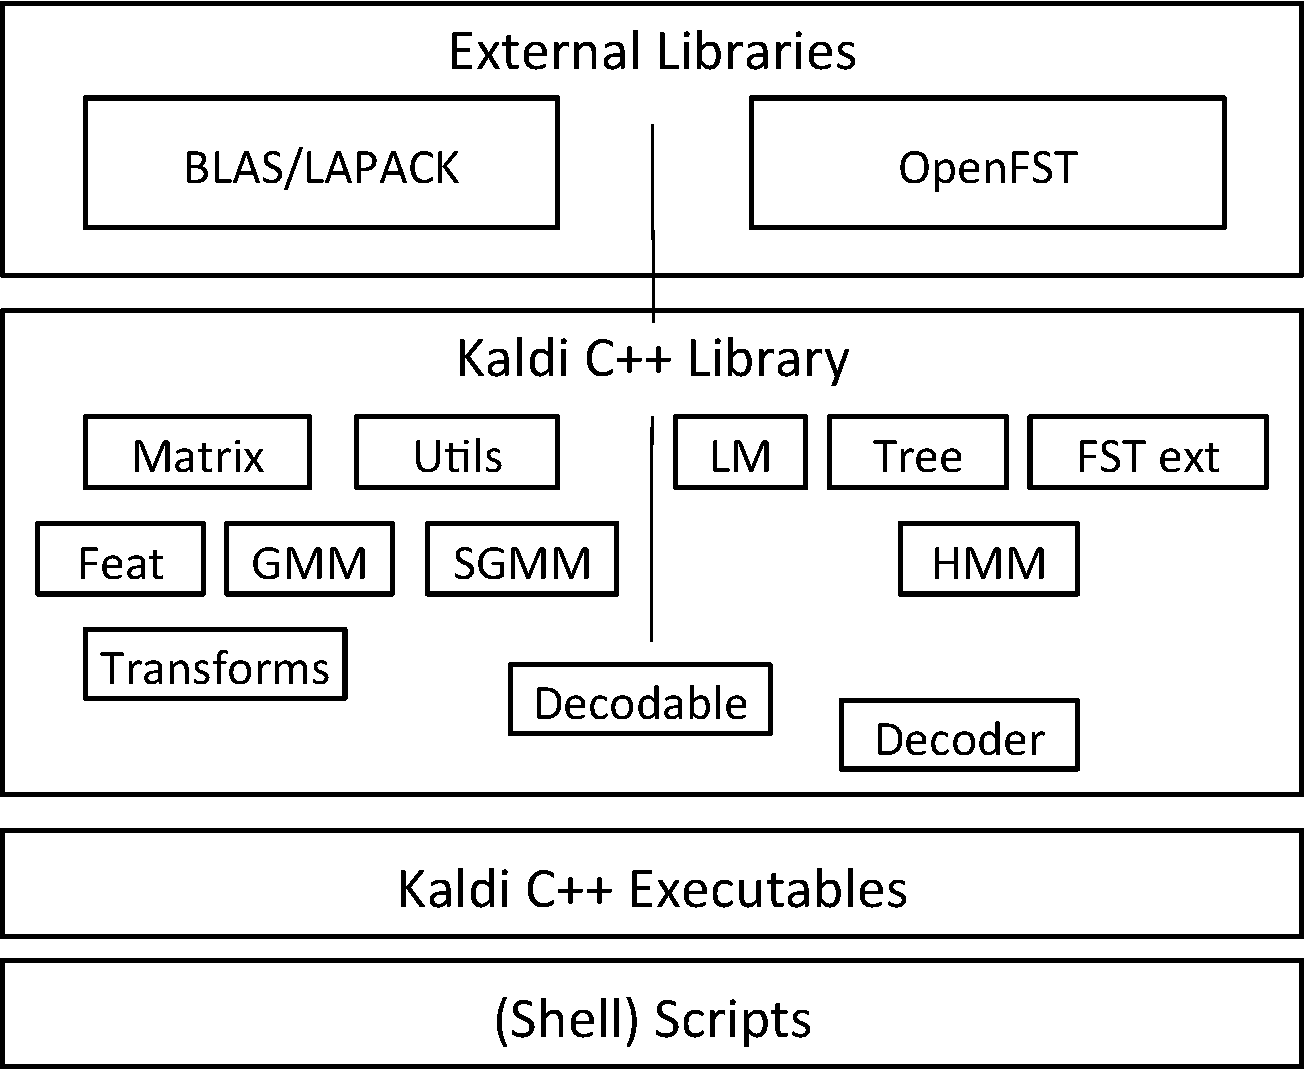
\includegraphics[width=0.75\columnwidth]{figs/kaldi-lib}\\
    \caption{A simplified view of the different components of Kaldi. The 
      library modules can be grouped into those that depend on linear algebra 
      libraries and those that depend on OpenFst. The {\em decodable} class 
      bridges these two halves. Modules that are lower down in the schematic 
      depend on one or more modules that are higher up.}
    \label{fig:kaldi-lib}
  \end{center}
\end{figure}

% We aim for the toolkit to be as loosely coupled as possible to make it easy 
% to reuse and refactor. This is reflected in the structure of the toolkit, where 
The library modules can be grouped into two distinct halves, each depending 
on only one of the external libraries (c.f. Figure \ref{fig:kaldi-lib}). A 
single module, the {\st DecodableInterface} (section \ref{sec:decoder}), 
bridges these two halves. 



Access to the library functionalities is provided through command-line tools 
written in C++, which are then called from a scripting language for building 
and running a speech recognizer. 
% While this is similar to the traditional approach followed in several toolkits (e.g. HTK), the Kaldi approach differs fundamentally in how we view the tools. 
Each tool has very specific functionality with a small set of command line 
arguments: for example, there are separate executables for accumulating 
statistics, summing accumulators, and updating a GMM-based acoustic model using 
maximum likelihood estimation. 
% As such the code for the executables tend to be very simple with only a small set of command line arguments. 
Moreover, all the tools can read from and write to pipes which makes it 
easy to chain together different tools.

To avoid ``code rot'', We have tried to structure the toolkit in such a way that
implementing a new feature will generally involve adding new code and
command-line tools rather than modifying existing ones.


% An approach that has recently become popular is to have a scripting
% language such as Python call the C++ code directly, and to have the outer-level
% control flow and system design done in this scripting language.  This is
% the approach used in IBM's Attila toolkit~\cite{attila}.  The design of
% Kaldi does not preclude doing this in future, but for now we have avoided
% this approach because it requires users to be proficient in two different
% programming languages.

%A final point to mention is that we tend to prefer provably correct 
%algorithms. There has been an effort to avoid recipes and algorithms that 
%could possibly fail, even if they don't fail in the ``normal case'' (for 
%example, FST weight-pushing, which normally helps but which can fail or make things 
%much worse in certain cases).

% % -------------------------------------------------------------------------
% % -------------------------------------------------------------------------
% \section{The Kaldi Matrix Library}
% \label{sec:matrix}
% The Kaldi matrix library provides C++ classes for vector and different types of 
% matrices (description follows), as well as methods for linear algebra routines, 
% particularly inner and outer products, matrix-vector and matrix-matrix 
% products, matrix inversions and various matrix factorizations like Cholesky 
% and singular value decomposition (SVD) that are required by 
% various parts of the toolkit. The library avoids operators in favor of function 
% calls, and requires the matrices and vectors to have correct sizes instead of 
% automatically resizing the outputs.

% The matrix library does not call the Fortran interface of BLAS and LAPACK
% directly, but instead calls their C-language interface in form of CBLAS and 
% CLAPACK. In particular, we have tested Kaldi using the ``Automatically Tuned 
% Linear Algebra Software'' (ATLAS) \cite{atlas} library, the 
% Intel Math Kernel Library (MKL) library, and the Accelerate 
% Framework on OS X. It is possible to compile Kaldi with only ATLAS, even though
% ATLAS does not provide some necessary LAPACK routines, like SVD and eigenvalue 
% decompositions. For those routines we use a C++ implementation of code from the 
% ``Java Matrix Package'' (JAMA) \cite{jama} project.

% % -------------------------------------------------------------------------
% \subsection{Matrix and vector types}
% The matrix library defines the basic {\st Vector} and {\st Matrix} classes, 
% which are templated on the floating point precision type ({\st float} or {\st 
% double}). 
% {\scriptsize
% \begin{verbatim}
% template<typename Real> class Vector;
% template<typename Real> class Matrix;
% \end{verbatim}}
% % // Symmetric packed matrix class:
% % template<typename Real> class SpMatrix;
% % // Triangular packed matrix class:
% % template<typename Real> class TpMatrix;
% The {\st Matrix} class corresponds to the general matrix (GE) in BLAS and 
% LAPACK. There are also special classes for symmetric matrices ({\st SpMatrix}) 
% and triangular matrices ({\st TpMatrix}) (for Cholesky factors). Both of these 
% are represented in memory as a ``packed'' lower-triangular matrix. Currently, 
% we only support linear algebra operations with real numbers, although it is 
% possible to extend the functionality to include complex numbers as well, since 
% the underlying BLAS and LAPACK routines support complex numbers also.

% For matrix operations that involve only part of a vector or matrix, the {\st 
% SubVector} and {\st SubMatrix} classes are provided, which are treated as a 
% pointer into the underlying vector or matrix. These inherit from a common base 
% class of {\st Vector} and {\st Matrix}, respectively, and can be used in any 
% operation that does not involve memory allocation or deallocation.


% % -------------------------------------------------------------------------
% % -------------------------------------------------------------------------
% \section{Finite State Transducer (FST) library}
% \label{sec:fstext}

% We compile and link against an OpenFst~\cite{openfst}, which is an open-source
% weighted finite-state transducer library.  Both our training and decoding code
% accesses WFSTs, which are simply OpenFst's C++ objects (we will sometimes
% refer to these just as FSTs).  

% We also provide code for various extensions to the OpenFst library, such as a
% constructed-on-demand context FST ($C$) which allows our toolkit to work
% efficiently for wide phonetic context.  There are also different versions of or
% extensions to some of the fundamental FST algorithms such as determinization,
% which we implement with epsilon removal and mechanisms to preserve stochasticity
% (discussed in Section~\ref{sec:graphs}); minimization, which we modify to work
% with non-deterministic input; and composition, where we provide a more efficient
% version.  We provide command-line tools with interfaces similar to OpenFst's
% command line tools, to allow these algorithms to be used from the shell.




% -------------------------------------------------------------------------
% -------------------------------------------------------------------------
% \section{Finite State Transducer Algorithms}
% \label{sec:fstext}


% % -------------------------------------------------------------------------
% \subsection{Determinization}

% We use a different determinization algorithm from the one in OpenFst. Our 
% determinization algorithm is actually closer to the standard FST 
% determinization algorithm than the one in OpenFst, in that it does epsilon 
% removal along with determinization (thus, like many other FST algorithms, we do 
% not consider epsilon to be a ``real symbol'').

% Our determinization algorithm has a different way of handling what happens when 
% a transition in the initial determinized output has more than one output symbol 
% on it. The OpenFst determinization algorithm uses a function that moves the 
% output symbols (encoded as weights) around while maintaining equivalence, 
% in order to ensure that no arc has more than one (encoded) output symbol; it 
% does not introduce new states with epsilon symbols on their input, which is the 
% most ``obvious'' thing to do. However, this algorithm can fail for the output 
% of our determinization algorithm, because there can be cycles with more outputs 
% than states on the cycle (because it does epsilon removal). Instead, whenever 
% we encounter a link with more than one output symbols, we create a chain with a 
% sufficient number of intermediate states to accommodate all the output symbols. 
% The weight and input symbol go on the first link of this chain. The output of 
% our DeterminizeStar algorithm is deterministic according to the definitions 
% OpenFst uses, i.e. treating epsilons as a normal symbols. Its output does have 
% epsilons on the input side, which is against the normal definition of 
% determinism, but this is to be viewed as an encoding mechanism for allowing 
% more than one output symbol on a link, and in any case it only happens in quite 
% specific circumstances (an epsilon arc is always the only arc out of a state).

% % One other difference is that our program fstdeterminizestar does not require 
% % the input FST to have its output symbols encoded as weights.

% We supply a function which casts an FST in the tropical semiring to the log 
% semiring before determinizing, and then converts back. This is the form of 
% determinization used in our algorithms, as it preserves stochasticity (see 
% Section \ref{sec:fst:stoch}).

% % -------------------------------------------------------------------------
% \subsection{Removing epsilons}

% We supply an epsilon-removal algorithm called {\st RemoveEpsLocal()} that is 
% guaranteed to never blow up the FST, but on the other hand is not guaranteed to 
% remove all epsilons. This function has slightly different behaviour from 
% OpenFst's {\st RemoveEps()} function, because it will combine two arcs if one 
% has an input epsilon and one an output epsilon. The function preserves FST 
% equivalence.

% There is also a function {\st RemoveEpsLocalSpecial()} that preserves 
% equivalence in the tropical semiring while preserving stochasticity in the log 
% semiring (for more on stochasticity see next section). This is a case where the 
% usefulness of the semiring formalism breaks down a little bit, as we have to 
% consider two semirings simultaneously.

% % -------------------------------------------------------------------------
% \subsection{Preserving stochasticity and testing it}
% \label{sec:fst:stoch}
% We define a stochastic FST as an FST in which, in the FST's semiring the sum of 
% the weights of the arcs out of any given state (plus the final-weight) equals 
% one (in the semiring). This concept is most useful and natural in the log 
% semiring; essentially, a stochastic FST is one where the sum of the weights out 
% of a given arc is one (e.g. a properly normalized HMM would correspond to a 
% stochastic FST).

% We aim for most of the FST algorithms we use to preserve stochasticity, in the 
% sense that they will produce stochastic outputs given stochastic inputs. For 
% non-stochastic inputs, we aim that the minimum and maximum range of the weights 
% will not get larger. In order to preserve stochasticity, the FSTs that we 
% compose with have to have certain properties. Consider L, for example. 
% We require that for any linear FST corresponding to a path through G, call this 
% FST F, the product L o F must be stochastic. This basically means that L have 
% properly normalized pronunciation probabilities. The actual property formally 
% required may be a little stronger than this (this relates to ensuring that the 
% probabilities appear at the ``right time''). 

% % -------------------------------------------------------------------------
% \subsection{Minimization}

% We use the minimization algorithm supplied by OpenFst, but we apply a patch 
% before compiling OpenFst so that minimization can be applied to 
% non-deterministic FSTs. The reason for this is so that we can remove 
% disambiguation symbols before minimizing, which is more optimal (it allows 
% minimization to combine more states). Fundamentally, OpenFst's minimization 
% algorithm is applicable to non-deterministic FSTs. This is 
% the same thing the fstminimize program does except that it does not do weight 
% pushing. This is desirable for us because the way we ensure stochasticity 
% entails avoiding any weight pushing.

% % -------------------------------------------------------------------------
% \subsection{Composition}

% For the most part we use OpenFst's own composition algorithms, but we do make 
% use of a more efficient composition algorithm for certain common cases. It uses 
% the ``Matcher'' concept of OpenFst; a Matcher is a kind of helper class used 
% during composition that performs lookup on the arcs out of a state to find any 
% arcs with a particular input or output symbol. The normal matcher that OpenFst 
% uses is SortedMatcher, which relies on arcs being sorted on the relevant label, 
% and does a binary search. TableMatcher detects cases where it would be 
% efficient to build a table indexed by label, and for those states it avoids the 
% overhead of binary search. This leads to a speedup when composing with things 
% like lexicons that have a very high out-degree.

% % -------------------------------------------------------------------------
% \subsection{Adding and removing disambiguation symbols}

% Our FST recipes (like other transducer-based recipes) rely on disambiguation 
% symbols. In the normal recipes, these are added to the input side of the 
% lexicon FST (L) to make it determizable. We also add disambiguation symbols to 
% G and C (see Disambiguation symbols). Whenever we do a composition and the FST 
% on the right has disambiguation symbols on its input, we (in theory) add to 
% each state in the left-hand FST a self-loop for each of the disambiguation 
% symbols, which has that symbol on both its input and output. Note that the 
% actual integer symbols id's for the disambiguation symbols on the left and 
% right may not be the same. For instance, we have a special symbol \#0 in G 
% (where epsilon would normally be). The symbol-id for this would generally be 
% the highest-numbered word plus one. But when we want to pass this symbol 
% through L, we need a symbol in L's input symbol table (which mainly contains 
% phones), to represent \#0. We have a function AddSelfLoops() that takes a 
% mutable FST and two vectors of labels (a label is an integer id for a symbol). 
% The vectors are the same size, and represent corresponding input and output 
% labels for the disambiguation symbols. This function adds self-loops to each 
% final state and each state with non-epsilon output symbols on at least one arc 
% out of it.

% We remove disambiguation symbols with the function DeleteISymbols(), accessible 
% on the command line with the program fstrmsymbols.


% -------------------------------------------------------------------------
% -------------------------------------------------------------------------
\section{Feature Extraction}
\label{sec:feats}
Our feature extraction and waveform-reading code aims to create standard MFCC 
and PLP features, setting reasonable defaults but leaving available the options 
that people are most likely to want to tweak (for example, the number of mel 
bins, minimum and maximum frequency cutoffs, etc.).  We support most commonly
used feature extraction approaches: e.g. VTLN, cepstral mean and variance normalization,
LDA, STC/MLLT, HLDA, and so on.

%The feature extraction 
%pipeline is implemented as a series of functions, each of which output a 
%matrix of floating point numbers and take a matrix as input, except the 
%windowing function, which reads the waveform samples as a vector. 

% The windowing function can optionally dither (add random Gaussian noise to) 
% the waveform, remove DC offset and pre-emphasize the higher frequencies. 
% Our FFT implementation~\cite{rico_book} works for window lengths that are not 
% powers of 2, and we also provide an implementation of split-radix FFT for 
% 0-padded windows whose lengths are powers of 2. 
% We support cepstral liftering 
% and optional warping of the Mel filter banks using vocal tract length 
% normalization (VTLN). 

%Cepstral mean and variance normalization, dynamic (i.e. 
%delta) features of arbitrary order, splicing of arbitrary number of frames 
% to the left or right of the current frame 
%and dimensionality reduction using linear discriminant analysis (LDA) or 
%heteroscedastic linear discriminant analysis (HLDA) \cite{hlda} are supported 
%at the executable layer. 
% through simple command line tools. 
%Additionally, we support reading and writing of features in the format used by 
%HTK \cite{htkbook}.


% -------------------------------------------------------------------------
% -------------------------------------------------------------------------
\section{Acoustic Modeling}
\label{sec:am}
Our aim is for Kaldi to support conventional models (i.e. diagonal GMMs) and 
Subspace Gaussian Mixture Models (SGMMs), but to also be easily extensible to 
new kinds of model. 
% Following the general design philosophy of Kaldi, the 
% acoustic modeling code is made up of classes with very specific functionality 
% that do not ``know anything'' about how they get used. For example, the {\st 
% DiagGmm} class just stores the parameters of a diagonal-covariance Gaussian 
% mixture model (together with accessors and mutators for the parameters) and 
% provides methods for likelihood computation. Estimation of GMMs is handled by a 
% separate class\footnote{In fact, different estimation classes are responsible 
% for different estimation algorithms, e.g. ML or MMI.} that accumulates the 
% sufficient statistics. 

% -------------------------------------------------------------------------
\subsection{Gaussian mixture models}
We support GMMs with diagonal and full covariance structures. Rather than 
representing individual Gaussian densities separately, we directly implement a 
GMM class that is parametrized by the {\em natural parameters}, i.e. means 
times inverse covariances and inverse covariances. The GMM classes also store 
the {\em constant} term in likelihood computation, which consist of all the 
terms that do not depend on the data vector. 
% In other words, the constant term is the likelihood of the zero vector.
Such an implementation is suitable for efficient log-likelihood computation 
with simple dot-products. 

% -------------------------------------------------------------------------
\subsection{GMM-based acoustic model}
The ``acoustic model'' class {\st AmDiagGmm} represents a collection of {\st DiagGmm} objects, indexed by ``pdf-ids'' that correspond to context-dependent
HMM states.   This class does not represent any HMM structure, but just a collection of densities (i.e. GMMs).
% with a slightly richer interface that supports, among other things, setting the number of Gaussian components in each pdf proportional to the occupancy of the corresponding HMM state. 
There are separate classes that represent the HMM structure, principally the 
topology and transition-modeling code and the code responsible for compiling 
decoding graphs, which provide a mapping between the HMM states and the pdf 
index of the acoustic model class.  
% The classes for estimating the acoustic model parameters are likewise implemented as a collection of GMM estimators. 
Speaker adaptation and other linear transforms like maximum likelihood linear 
transform (MLLT) \cite{mllt} or semi-tied covariance (STC) \cite{stc} are 
implemented by separate classes.

% -------------------------------------------------------------------------
\subsection{HMM Topology}
It is possible in Kaldi to separately specify the HMM topology for each 
context-independent phone.  The topology format allows nonemitting states, and 
allows the user to pre-specify tying of the p.d.f.'s in different HMM states. 

% -------------------------------------------------------------------------
\subsection{Speaker adaptation}
We support both model-space adaptation using maximum likelihood linear 
regression (MLLR) \cite{mllr} and feature-space adaptation using feature-space
MLLR (fMLLR), also known as constrained MLLR \cite{gales_linxform}. For both 
MLLR and fMLLR, multiple transforms can be estimated using a regression tree 
\cite{regtree}. When a single fMLLR transform is needed, it can be used as an 
additional processing step in the feature pipeline. 
% It is also possible to only estimate the bias vector of an affine transform, 
% or the bias vector and a diagonal transform matrix, which are suitable when 
% the amount of adaptation data is small\footnote{This is currently implemented only for fMLLR.}. 
The toolkit also supports speaker normalization using a linear approximation 
to VTLN, similar to \cite{lvtln}, or conventional feature-level VTLN, or
a more generic approach for gender normalization which we call the ``exponential 
transform''~\cite{asru_et}.  Both fMLLR and VTLN can be used for speaker adaptive training (SAT) of the acoustic models. 

% -------------------------------------------------------------------------
\subsection{Subspace Gaussian Mixture Models}
For subspace Gaussian mixture models (SGMMs), the toolkit provides an 
implementation of the approach described in \cite{sgmm_csl}. There is a single 
class {\st AmSgmm} that represents a whole collection of pdf's; unlike the 
GMM case there is no class that represents a single pdf of the SGMM. Similar to 
the GMM case, however, separate classes handle model estimation and speaker 
adaptation using fMLLR.

% -------------------------------------------------------------------------
% -------------------------------------------------------------------------
\section{Phonetic Decision Trees}
\label{sec:tree}
Our goals in building the phonetic decision tree code were to make it
efficient for arbitrary context sizes (i.e. we avoided enumerating
contexts), and also to make it general enough to support a wide range of
approaches.  The conventional approach is, in each HMM-state of each
monophone, to have a decision tree that asks questions about, say, 
the left and right phones.  In our framework, the decision-tree
roots can be shared among the phones and among the states of the
phones, and questions can be asked about any phone in the context window,
and about the HMM state.  Phonetic questions can be supplied based on
linguistic knowledge, but in our recipes the questions are generated
automatically based on a tree-clustering of the phones. 
Questions about things like phonetic stress (if marked in the dictionary)
and word start/end information are supported via an extended phone set;
in this case we share the decision-tree roots among the different versions of the
same phone.


% -------------------------------------------------------------------------
% -------------------------------------------------------------------------
\section{Language Modeling}
\label{sec:lm}
Since Kaldi uses an FST-based framework, it is possible, in principle, to use 
any language model that can be represented as an FST. 
% We are working on mechanisms that are able to handle LMs that would get too 
% large when represented this way. 
We provide tools for converting LMs in the standard ARPA 
format to FSTs.  In our recipes, we have used the IRSTLM toolkit
\footnote{Available from: http://hlt.fbk.eu/en/irstlm} for 
purposes like LM pruning.  For building LMs from raw text, users may use the 
IRSTLM toolkit, for which we provide installation help, or a more fully-featured
toolkit such as SRILM~\footnote{Available from: http://www.speech.sri.com/projects/srilm/}.

% -------------------------------------------------------------------------
% -------------------------------------------------------------------------
\section{Creating Decoding Graphs}
\label{sec:graphs}

All our training and decoding algorithms use Weighted Finite State Transducers 
(WFSTs).  In the conventional 
recipe~\cite{wfst}, the input symbols on the decoding graph correspond to 
context-dependent states (in our toolkit, these symbols are 
numeric and we call them pdf-ids).  However, because we allow different phones 
to share the same pdf-ids, we would have a number of problems with this 
approach, including not being able to determinize the FSTs, and not having 
sufficient information from the Viterbi path through an FST to work out the 
phone sequence or to train the transition probabilities.  In order to fix these 
problems, we put on the input of the FSTs a slightly more fine-grained integer 
identifier that we call a ``transition-id'', that encodes the pdf-id, the phone 
it is a member of, and the arc (transition) within the topology specification 
for that phone.  There is a one-to-one mapping between the ``transition-ids'' 
and the transition-probability parameters in the model: we decided 
make transitions as fine-grained as we could without increasing the 
size of the decoding graph.  
%An advantage of having the transition-ids as the 
%graph input symbols is that all we need in Viterbi-based model training is the 
%sequence of input symbols (transition-ids) in the Viterbi path through the 
%FST.  We call this sequence an alignment.  A set of alignments gives us all the 
%information we need in order to train the p.d.f.'s and the transition 
%probabilities.  Since an alignment encodes the complete phone sequence, it is 
%possible to convert alignments between different decision trees.

Our decoding-graph construction process is based on the recipe described
in~\cite{wfst}; however, there are a number of differences.  One important one
relates to the way we handle ``weight-pushing'', which is the operation that is
supposed to ensure that the FST is stochastic.  ``Stochastic'' means that the
weights in the FST sum to one in the appropriate sense, for each state (like a
properly normalized HMM).  Weight pushing may fail or may lead to bad pruning 
behavior if the FST representing the grammar or language model ($G$) is not 
stochastic, e.g. for backoff language models.  Our approach is to
avoid weight-pushing altogether, but to ensure that each stage of graph creation
``preserves stochasticity'' in an appropriate sense.  Informally, what this 
means is that the ``non-sum-to-one-ness'' (the failure to sum to one) will 
never get worse than what was originally present in $G$. 

% This requires changes 
%to some algorithms, e.g. determinization.  

%There are other 
%differences too: we minimize after removing disambiguation symbols, which is 
%more optimal but requires changes to the minimization code of OpenFst; and we 
%use a version of determinization that removes input epsilon symbols, which 
%requires certain changes in other parts of the recipe (chiefly: introducing 
%disambiguation symbols on the input of $G$).

% The graph creation process required in test time is put together at the 
% shell-script level.  In training 
% time, the graph creation is done as a C++ program which can be made more 
% efficient.  The aim is for all the C++ tools to be quite generic, and not to 
% have to know about ``special'' things like silence.  For instance, alternative 
% pronunciations and optional silence are supplied as part of the lexicon FST 
% ($L$) which is generally produced by a script.

% -------------------------------------------------------------------------
% -------------------------------------------------------------------------
\section{Decoders}
\label{sec:decoder}
We have several decoders, from simple to highly optimized; more will be added 
to handle things like on-the-fly language model rescoring and lattice 
generation.  By ``decoder'' we mean a C++ class that implements the core 
decoding algorithm.  The decoders do not require a particular type of acoustic 
model: they need an object satisfying a very simple interface with a function 
that provides some kind of acoustic model score for a particular (input-symbol 
and frame).  

{\scriptsize
\begin{verbatim}
class DecodableInterface {
 public:
  virtual float LogLikelihood(int frame, int index) = 0;
  virtual bool IsLastFrame(int frame) = 0;
  virtual int NumIndices() = 0;
  virtual ~DecodableInterface() {}
};
\end{verbatim}}

Command-line decoding programs are all quite simple, do just one 
pass of decoding, and are all specialized for one decoder and one 
acoustic-model type.  Multi-pass decoding is implemented at the script level.



% -------------------------------------------------------------------------
% -------------------------------------------------------------------------
\section{Experiments}
\label{sec:expt}
We report experimental results on the Resource Management (RM) corpus and on 
Wall Street Journal.  
% We note that the experiments reported here should be fully reproducible, 
% except for minor differences in WER due to differences in compiler behavior 
% and random number generation algorithms.  
The results reported here correspond to version 1.0 of Kaldi; the scripts that 
correspond to these experiments may be found in {\st egs/rm/s1} and 
{\st egs/wsj/s1}.

% and we will provide ``system identifiers'' (corresponding to 
%training runs) to help locate particular experiments in our scripts.

% The scripts include all data preparation stages, and require only the 
% original datasets as distributed by the Linguistic Data Consortium (LDC).

% %% Arnab, if you don't like this format, we can discuss other options.
% {\scriptsize
% \begin{verbatim}
% svn co \
%  https://kaldi.svn.sourceforge.net/svnroot/kaldi/kaldi-v1.0
% \end{verbatim}
% }

% ; see
% {\scriptsize \verb|egs/rm/README.txt|} and {\scriptsize \verb|egs/wsj/README.txt|}.
% In the experimental results in this section we will provide system identifiers
% to make it easier to locate the corresponding experiments.

\subsection{Comparison with previously published results}

% We first report some results intended to demonstrate that the basic
% algorithms included in the toolkit give results comparable to those
% previously reported in the literature.

\begin{table}
\centering{
  \caption{Basic triphone system on Resource Management: \%WERs}
  \label{rm:baseline}
  \begin{tabular}{|c|c|c|c|c|c|} \hline
           & \multicolumn{5}{|c|}{    Test set  }   \\ \cline{2-6}
           &  Feb'89 &  Oct'89 & Feb'91 & Sep'92 & Avg   \\ \hline
    HTK    &  2.77    &  4.02   &  3.30  &  6.29  &  4.10 \\
    Kaldi  &  3.20    &  4.21   &  3.50  &  5.86  &  4.06 \\ \hline 
  \end{tabular}}
\end{table}

Table~\ref{rm:baseline} shows the results of a context-dependent triphone system
with mixture-of-Gaussian densities; the HTK baseline numbers are taken 
from~\cite{Povey:ICASSP99} and the systems use essentially the same algorithms.
The features are MFCCs with per-speaker cepstral mean subtraction.  The language
model is the word-pair bigram language model supplied with the RM corpus.
The WERs are essentially the same.  Decoding time was about 0.13$\times$RT, measured
on an Intel Xeon CPU at 2.27GHz.  The system identifier for the Kaldi results is
tri3c.

Table~\ref{wsj:baseline} shows similar results for the Wall Street Journal 
system, this time without cepstral mean subtraction.  The WSJ corpus comes with
bigram and trigram language models.
% and most of our experiments use a pruned version of the trigram language model (with the number of entries reduced from 6.7 million to 1.5 million) since our 
% fully-expanded FST gets too large with the full language model (we are working on decoding strategies that can work with large language models).  
% For comparison with published results, we report bigram
% decoding in Table~\ref{wsj:baseline}, 
and we compare with published numbers using the bigram language model. The 
baseline results are reported in~\cite{Reichl:ITSAP00}, which we refer to as 
``Bell Labs'' (for the authors' affiliation), and a HTK system described 
in~\cite{Woodland:ICASSP94}.  The HTK system was gender-dependent (a gender-independent
baseline was not reported), so the HTK results are slightly better.  Our decoding
time was about 0.5$\times$RT.

\begin{table}
\centering{
 \caption{Basic triphone system, WSJ, 20k open vocabulary, bigram LM, SI-284 train: \%WERs}
 \label{wsj:baseline}
\begin{tabular}{|c|c|c|} \hline
            & \multicolumn{2}{|c|}{    Test set  }   \\ \cline{2-3}
            &  Nov'92      &    Nov'93  \\ \hline
  Bell      &  11.9        &  15.4    \\
 HTK (+GD)  &  11.1        &  14.5   \\ 
 KALDI      &  11.8        &  15.0   \\ \hline
\end{tabular}}
\end{table}


\subsection{Other experiments}

Here we report some more results on both the WSJ test sets (Nov'92 and Nov'93) 
using systems trained on just the SI-84 part of the training data, that
demonstrate different features that are supported by Kaldi. 
% Note that the triphone results for the WSJ sets are worse than those in Table 
% \ref{wsj:baseline} due to the smaller training set. 
We also report results on the RM task, averaged over 6 test sets: the 4 
mentioned in table \ref{rm:baseline} together with Mar'87 and Oct'87. The best 
result for a conventional GMM system is achieved by a SAT 
% a speaker-adaptively trained 
system that splices 9 frames (4 on each side of the 
current frame) and uses LDA to project down to 40 dimensions, together with 
MLLT.  We achieve better performance on average, with an SGMM system trained
on the same features, with speaker vectors and fMLLR adaptation.  The last
line, with the best results, includes the ``exponential transform''~\cite{asru_et} in
the features.

\begin{table}
\centering{
 \caption{Results on RM and on WSJ, 20k open vocabulary, bigram LM, trained on half of SI-84: \%WERs}
 \label{results}
\begin{tabular}{|l|c|c|c|} \hline
                             & RM (Avg) & WSJ Nov'92 & WSJ Nov'93 \\ \hline
 Triphone                    & 3.97     & 12.5       &  18.3   \\
 \,\, + fMLLR                & 3.59     & 11.4       &  15.5   \\ 
 \,\, + LVTLN                & 3.30     & 11.1       &  16.4   \\ 
 Splice-9 + LDA + MLLT       & 3.88     & 12.2       &  17.7   \\ 
 \,\, + SAT (fMLLR)          & 2.70     & 9.6        &  13.7   \\ 
 \,\, + SGMM + spk-vecs      & 2.45     & 10.0       &  13.4   \\ 
 \qquad + fMLLR              & 2.31     & 9.8        &  12.9   \\ 
 \qquad + ET                 & 2.15     & 9.0        &  12.3   \\
\hline
\end{tabular}}
\end{table}

% -------------------------------------------------------------------------
% -------------------------------------------------------------------------
\section{Conclusions}
\label{sec:conclusion}
We described the design of Kaldi, a free and open-source speech recognition 
toolkit. The toolkit currently supports modeling of context-dependent phones of 
arbitrary context lengths, and all commonly used techniques that can be 
estimated using maximum likelihood. It also supports the recently proposed 
SGMMs. Development of Kaldi is continuing and we are working on using large 
language models in the FST framework, lattice generation and discriminative 
training.

% -------------------------------------------------------------------------
% -------------------------------------------------------------------------
\section*{Acknowledgments}

{\footnotesize
We would like to acknowledge participants and collaborators in the 2009 Johns
Hopkins University Workshop, including Mohit Agarwal, Pinar Akyazi, Martin
Karafiat, Feng Kai, Ariya Rastrow, Richard C. Rose and Samuel Thomas; Patrick
Nguyen, for introducing the participants in that workshop and for help with WSJ
recipes, and faculty and staff at JHU for their help during that workshop, 
including Sanjeev Khudanpur, Desir\'{e}e Cleves, and the late Fred Jelinek.  

We would like to acknowledge the support of Geoffrey Zweig and Alex Acero at 
Microsoft Research.  We are grateful to Jan (Honza) \v{C}ernock\'{y} 
for helping us organize the workshop at the Brno University of Technology 
during August 2010 and 2011. Thanks to Tomas Ka\v{s}p\'{a}rek for system 
support and Renata Kohlov\'{a} for administrative support.  

We would like to thank Michael Riley, who visited us in Brno to deliver 
lectures on finite state transducers and helped us understand OpenFst; Henrique 
(Rico) Malvar of Microsoft Research for allowing the use of his FFT code; and 
Patrick Nguyen for help with WSJ recipes. 
We would like to acknowledge the help with coding and documentation from 
Sandeep Boda and Sandeep Reddy (sponsored by Go-Vivace Inc.) and Haihua Xu.  
We thank Pavel Matejka (and Phonexia s.r.o.) for allowing the use of feature 
processing code. 

% It is possible that this list of contributors contains oversights; any 
% important omissions are unlikely to be intentional.

During the development of Kaldi, Arnab Ghoshal was supported by the European 
Community's Seventh Framework Programme under grant agreement no. 213850 
(SCALE); the BUT researchers were supported by the Technology Agency of the 
Czech Republic under project No. TA01011328, and partially by Czech MPO project 
No. FR-TI1/034. 

The JHU 2009 workshop was supported by National Science Foundation Grant Number
IIS-0833652, with supplemental funding from Google Research, DARPA's GALE program
and the Johns Hopkins University Human Language Technology Center of Excellence.

% Finally, it is quite possible that someone else who helped us significantly was
% inadvertently omitted here; if so, we apologize.
}

\bibliographystyle{IEEEtran}
\bibliography{refs}

\end{document}

% LocalWords:  Kaldi automata OpenFst SGMM SourceForge toolkits HTK RWTH FST LM
% LocalWords:  BLAS LAPACK PACKage decodable refactor DecodableInterface GMM Xu
% LocalWords:  functionalities executables Cholesky SVD Fortran CBLAS CLAPACK
% LocalWords:  MKL JAMA templated SpMatrix TpMatrix SubVector SubMatrix WFSTs
% LocalWords:  deallocation OpenFst's FSTs determinization stochasticity MFCC
% LocalWords:  PLP mel pre FFT cepstral liftering VTLN LDA heteroscedastic HLDA
% LocalWords:  GMMs SGMMs DiagGmm accessors mutators MMI AmDiagGmm pdf MLLT STC
% LocalWords:  nonemitting fMLLR AmSgmm pdf's triphones monophone biphone LMs
% LocalWords:  ARPA IRSTLM SRILM determinize backoff rescoring WER egs triphone
% LocalWords:  WERs MFCCs bigram xRT spk LVTLN vecs WSJ Mohit Agarwal Pinar Ka
% LocalWords:  Akyazi Karafiat Feng Ariya Rastrow Sanjeev Khudanpur Desir Boda
% LocalWords:  Cleves Henrique Malvar Sandeep Reddy Haihua Matejka Phonexia rek
% LocalWords:  Zweig Acero Honza ernock Kohlov MPO IIS DARPA's
